\chapter{Исследовательская часть}

\section{Цель и условия исследования}

Цель исследования -- определить, как меняется время запроса поиска при наличии индекса по городу и дате и без него для 1000, 2000, 5000 и 10000~мероприятий. Использован запрос метода \texttt{SearchEvents}, который соединяет мероприятие с локацией, исключает удаленные объявления, применяет фильтры и сортирует результат по дате и идентификатору. Загрузка категорий, участников и авторов после основного запроса не измерялась.

В обоих вариантах заданы город Москва и интервал от 26.08.2026 до 25.10.2026; фильтры названия и категорий не заданы. Опорная дата набора данных -- 25.09.2026. Четыре объема являются вложенными частями одного сгенерированного набора. Число локаций постоянно и равно 12006; около 5\% мероприятий помечены удаленными.

Исследуемый индекс имеет те же поля и условие, что и индекс приложения \texttt{event\_search\_city\_date\_idx}:

\begin{verbatim}
create index research_city_date_idx
    on event (city, event_date, id)
    where deleted = false;
\end{verbatim}

Поле \texttt{city} отвечает условию равенства, \texttt{event\_date} -- диапазону дат, а \texttt{id} входит в порядок сортировки. Вариант без исследуемого индекса сохраняет первичный ключ временной таблицы; сравнивается действие именно этого дополнительного индекса.

Измерения проводились на компьютере с процессором AMD~Ryzen~7~7700 и 32~ГБ оперативной памяти под управлением Windows~11. PostgreSQL~16.11 работала в WSL2; для выполнения запросов использовалась библиотека \texttt{psycopg}~3.3.6. Данные размещены во временных таблицах. Параллельное выполнение и JIT отключены; планировщику заданы \texttt{shared\_buffers}~128~МиБ, \texttt{work\_mem}~4~МиБ и \texttt{random\_page\_cost=4}. Кеш перед измерениями прогревался и не сбрасывался. В сохраненном протоколе указаны 12~логических процессоров, доступных среде WSL2.

\section{Методика измерения}

Для каждой комбинации объема данных и наличия индекса проведено 10~блоков по 50~измерений. Перед каждым блоком выполнено 10~прогревочных запросов. Порядок вариантов с индексом и без него чередовался между блоками. Таким образом, на каждую точку графика приходится 500~измерений, всего получено 4000~измерений. Все значения включены в расчет среднего.

Измеряемая величина -- серверное время \texttt{Execution Time} команды \texttt{EXPLAIN (ANALYZE, BUFFERS, TIMING OFF, FORMAT JSON)}. Время планирования записано отдельно и в результат не входит. Среднее вычислено по 500~значениям. Погрешность на графике и в таблице рассчитана как $2{,}262s/\sqrt{10}$, где $s$ -- выборочное стандартное отклонение десяти средних значений по блокам. Это оценка 95\%-го доверительного интервала при независимости блоков; из-за возможной корреляции блоков ее следует использовать только для ориентировочного сравнения.

\section{Результаты исследования}

Средние значения из 4000~исходных строк протокола приведены в таблице~\ref{tab:research-results}. Число найденных строк при каждом объеме одинаково для обоих вариантов.

\begin{table}[H]
    \caption{Время выполнения запроса поиска}
    \label{tab:research-results}
    \small
    \begin{tabularx}{\textwidth}{|p{2.0cm}|Y|Y|p{2.1cm}|}
        \hline
        \textbf{Записей} & \textbf{Без индекса, мс} & \textbf{С индексом, мс} & \textbf{Найдено} \\
        \hline
        1000 & $0{,}325 \pm 0{,}005$ & $0{,}199 \pm 0{,}004$ & 57 \\
        \hline
        2000 & $1{,}824 \pm 0{,}054$ & $1{,}583 \pm 0{,}077$ & 105 \\
        \hline
        5000 & $2{,}673 \pm 0{,}080$ & $1{,}973 \pm 0{,}043$ & 287 \\
        \hline
        10000 & $4{,}905 \pm 0{,}320$ & $3{,}038 \pm 0{,}203$ & 600 \\
        \hline
    \end{tabularx}
\end{table}

Зависимость времени от числа мероприятий представлена на рисунке~\ref{fig:research-index}. Сплошная линия с кругами соответствует варианту без индекса, пунктирная с квадратами -- варианту с индексом; обозначения различимы при черно-белой печати.

\begin{figure}[H]
    \centering
    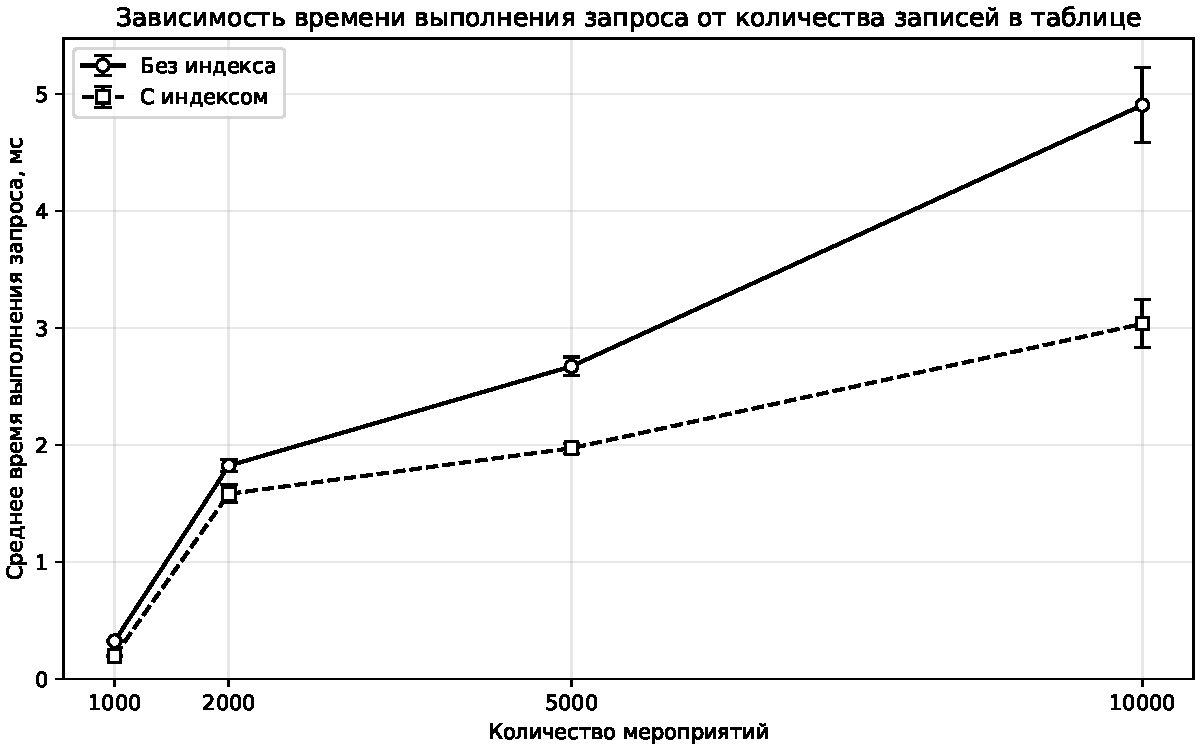
\includegraphics[width=0.95\textwidth]{../app/scripts/index_chart.pdf}
    \caption{Зависимость времени поиска от числа мероприятий}
    \label{fig:research-index}
\end{figure}

В сохраненных планах запрос без дополнительного индекса сканирует таблицу \texttt{event} последовательно. При наличии индекса применяется \texttt{Bitmap Index Scan} с последующим \texttt{Bitmap Heap Scan}. Для 1000~мероприятий соединение с \texttt{location} выполнено вложенным циклом, для остальных объемов -- хеш-соединением. Смена способа соединения может влиять на рост времени между 1000 и 2000~строками; считать ее единственной причиной нельзя.

\section*{Вывод}

Во всех четырех наборах среднее время с индексом меньше, чем без него. Для 10000~мероприятий оно составило 3,038~мс вместо 4,905~мс, то есть сократилось примерно на 38\%. Результат относится к одному SQL-запросу, заданным фильтрам, синтетическим данным и прогретому кешу временных таблиц. Он не характеризует время загрузки страницы или работу всего приложения под нагрузкой.
